\section{Kiến trúc phần mềm}

Ngày nay, có rất nhiều mô hình kiến trúc hệ thống để cho chúng tôi lựa chọn.
Tuy nhiên, chúng tôi ưu tiên lựa chọn mô hình kiến trúc phần mềm có khả năng
tương thích với hệ thống cũ, độ tin cậy cao, độ mở rộng cao và đơn giản, phù hợp với
kích thước của hệ thống. Chúng tôi xem xét hai loại kiến trúc rất phổ biến hiện nay, đó là 
kiến trúc đa lớp và kiến trúc microservices.

\par
Kiến trúc đa lớp là một trong những kiến trúc phổ biến trong các loại kiến trúc phần mềm. Kiến trúc
này ra đời nhằm phân chia các thành phần trong hệ thống, các thành phần cùng
chức năng sẽ được nhóm lại với nhau và phân chia công việc cho từng nhóm để dữ
liệu không bị chồng chéo và lộn xộn. Kiến trúc này phát huy hiệu quả nhất ở cả hệ 
thống nhỏ và lớn, giúp cho việc quản lý code và xử lý lỗi dễ
dàng hơn.
\par
Mặc dù không có quy định cụ thể về số lượng hay kiểu của các lớp, ở những hệ
thống phức tạp hơn có thể có nhiều lớp hơn, đa số các kiến trúc đa lớp gồm có
ba lớp chuẩn (3-tier): \emph{Presentation Layer}, \emph{Business Layer},
\emph{Persistence Layer}. \emph{Presentation layer} có nhiệm vụ chính giao tiếp với
người dùng, gồm các thành phần giao diện và thực hiện các công việc như nhập
liệu, hiển thị dữ liệu, kiểm tra tính đúng đắn của dữ liệu trước khi gọi lớp
\emph{Business layer}. \emph{Business layer} phân ra thành hai nhiệm vụ: thứ
nhất, đây là nơi đáp ứng các yêu cầu thao tác dữ liệu của \emph{Presentation
    layer}, xử lý chính nguồn dữ liệu từ \emph{Presentation layer} trước khi truyền
xuống \emph{Persistence layer} và lưu xuống hệ quản trị cơ sở dữ liệu. \emph{Persistence 
layer} có chức năng giao tiếp với hệ quản trị cơ sở dữ liệu như thực hiện các công việc
liên quan đến lưu trữ và truy vấn dữ liệu ( tìm kiếm, thêm, xóa, sửa,…).
\begin{figure}[H]
    \centering
    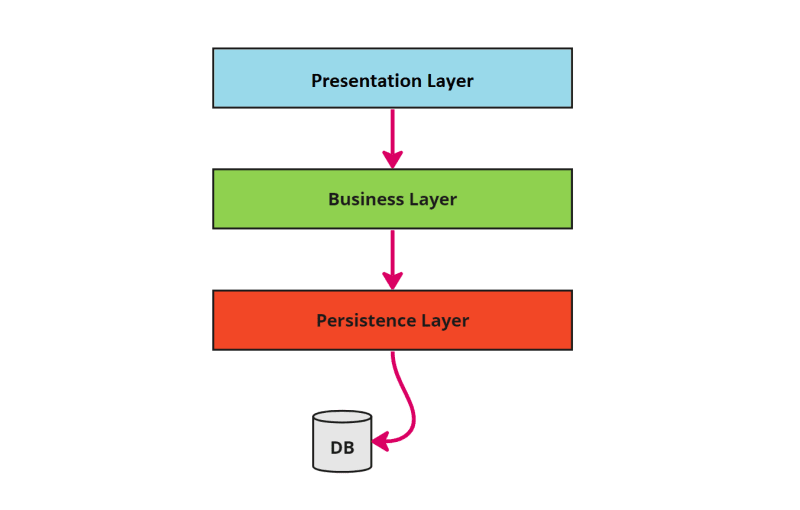
\includegraphics[width=\linewidth]{Content/Phân tích và thiết kế hệ thống/documents/Kiến trúc hệ thống/images/n tier architecture.png}
    \vspace{0.5cm}
    \caption{Mô hình kiến trúc đa lớp [6]}
    \label{fig:Mô hình kiến trúc đa lớp}
\end{figure}
\par
Kiến trúc này có một số ưu điểm như sau:
\begin{itemize}
    \item Việc phân chia thành từng lớp giúp cho code được tường minh hơn. Nhờ vào việc
          chia ra từng lớp đảm nhận các chức năng khác nhau và riêng biệt như giao diện,
          xử lý, truy vấn thay vì để tất cả lại một chỗ, nhằm giảm sự kết dính.
    \item Dễ bảo trì khi được phân chia, thì một thành phần của hệ thống sẽ dễ thay đổi.
          Việc thay đổi này có thể được cô lập trong 1 lớp, hoặc ảnh hưởng đến lớp gần
          nhất mà không ảnh hưởng đến cả chương trình.
    \item Dễ phát triển, tái sử dụng: khi chúng ta muốn thêm một chức năng nào đó thì
          việc lập trình theo một mô hình sẽ dễ dàng hơn vì chúng ta đã có chuẩn để tuân
          theo. Và việc sử dụng lại khi có sự thay đổi giữa hai môi trường thì chỉ việc
          thay đổi lại \emph{Presentation layer}.
      \item Phù hợp với các hệ thống vừa và nhỏ, với sự tăng trưởng nhỏ và có thể dự đoán được.
\end{itemize}

\par
Ngoài kiến trúc đa lớp này, chúng tôi còn tìm hiểu thêm một loại kiến trúc cũng
rất phổ biến hiện nay, đó là Microservices. Theo kiến trúc này, một ứng dụng
được chia thành một bộ các microservice, mỗi microservice thực chất là một
service có thể được triển khai và chạy độc lập. Chúng tách biệt về mặt mã
nguồn, về hoạt động và dữ liệu. Mỗi microservice có nơi chứa dữ liệu của riêng
của nó và chỉ có nó có quyền truy cập vào vùng dữ liệu này. Do các microservice
là độc lập, chúng không giao tiếp trực tiếp với nhau mà qua một thành phần
trung gian được gọi là \acrshort*{api} gateway. Có thể thấy vai trò của API gateway rất
quan trọng trong mô hình microservice. Nó là điểm đến và đi của mọi yêu cầu hay
phản hồi.
\begin{figure}[H]
      \centering
      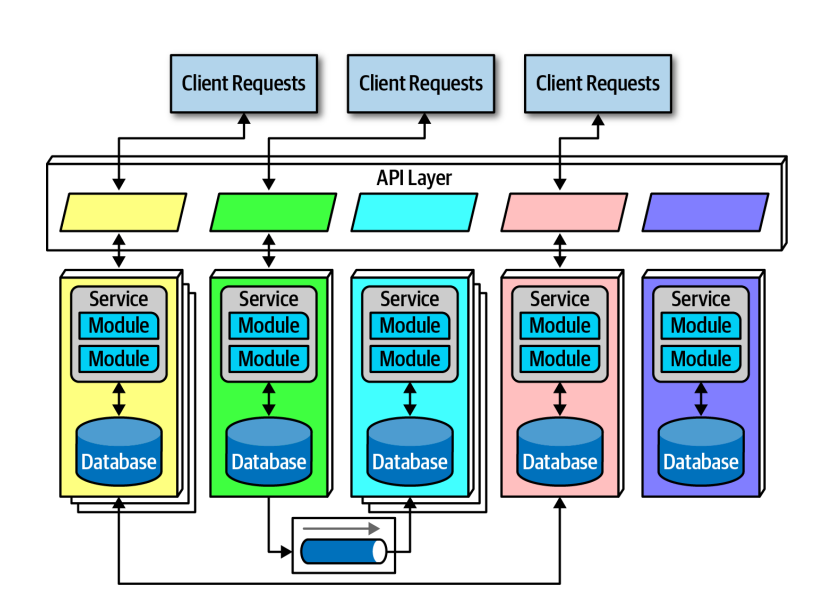
\includegraphics[width=\linewidth]{Content/Phân tích và thiết kế hệ thống/documents/Kiến trúc hệ thống/images/microservice.png}
      \vspace{0.5cm}
      \caption{Mô hình kiến trúc Microservices [10]}
      \label{fig:Mô hình kiến trúc Microservices}
\end{figure}
\par
Tính phân tán là đặc trưng của kiến trúc này, vì vậy việc xác định mức độ chi
tiết của từng dịch vụ là chìa khóa để xây dựng một hệ thống tốt. Đó là điều khó
đạt được đối với hệ thống đang phát triển của chúng tôi. Một vấn đề khác với
hướng tiếp cận theo kiến trúc này đó là việc các nghiệp vụ trong hệ thống chúng
tôi liên quan khá chặt chẽ, vì vậy kiến trúc Microservices tỏ ra không phù hợp
với hệ thống của chúng tôi.
\par
Với những phân tích trên về hai loại kiến trúc, chúng tôi quyết định sử dụng kiến
trúc đa lớp cho hệ thống của mình, không chỉ vì tính đơn giản, dễ hiểu mà còn vì
nó còn tương thích tốt hơn với hệ thống cũ cũng đang sử dụng loại hình kiến trúc này.